%%
%% neuralfields.tex
%% 
%% Made by jjfigueredou
%% Login   <jjfigueredou@fctp-jjfu>
%% 
%% Started on  Sun Oct  5 12:26:22 2008 jjfigueredou
%% Last update Sun Oct  5 12:26:22 2008 jjfigueredou
%%

\documentclass{sig-alt-release2}

\usepackage{algorithm}
\usepackage{algorithmic}

\begin{document}

\conferenceinfo{GECCO'09,} {July 8--12, 2009, Montr\'eal Qu\'ebec,
  Canada.}

\CopyrightYear{2009}

\crdata{978-1-60558-325-9/09/07}
%
% --- Author Metadata here --- \conferenceinfo{WOODSTOCK}{'97 El Paso,
%   Texas USA}
% \CopyrightYear{2007} % Allows default copyright year (200X) to be over-ridden - IF NEED BE.
% \crdata{0-12345-67-8/90/01} % Allows default copyright data (0-89791-88-6/97/05) to be over-ridden - IF NEED BE.
% --- End of Author Metadata ---

\title{Evolved Neural Fields Applied to the Stability Problem of a
  Simple Biped Walking Model}

\numberofauthors{1}
\author{\alignauthor Juan J. Figueredo, Jonatan G�mez \\
  \affaddr{Universidad Nacional de Colombia}
  \\ \affaddr{ Ciudad Universitaria, Bogot�, Colombia} \\
  \email{jjfigueredou@unal.edu.co, jgomezpe@unal.edu.co} }

\maketitle

\begin{abstract}
  This paper proposes an evolved control architecture based on neural
  fields for a relatively complex and unstable dynamical system. The
  neural field model is capable of addressing goal-based planning
  problems and has properties, like embedding in an Euclidean space
  and linear stability, that potentially make it well-fitted for
  dynamic control tasks. The neural field control architecture is
  tested over the stability problem on a typical inverted-pendulum and
  the performance of an evolved neural field and a hand-tuned neural
  field is compared. The neural field controller performs well in the
  simulation and has a spatial representation which allows
  interpretation of field potentials. Also, the evolved neural field
  performs almost as good as the non-evolved one, is more general, and
  uses a different strategy to control the plant.
\end{abstract}

\vspace{1mm}
\noindent {\bf Categories and Subject Descriptors:} I.2.8 {Artificial
  Intelligence}: {Problem Solving, Control Methods, and
  Search} 

\vspace{1mm}
\noindent {\bf General Terms:} Algorithms, Design.

\vspace{1mm}
\noindent {\bf Keywords:} Neural fields, neurocontrol, evolutionary
robotics.

\section{Introduction}
In biped robotics, the methods based on computational intelligence for
planning and control have shown to be able to achieve static stability,
% \cite{Kun97Adaptive}
 dynamical stability
% \cite{Nakanishi2004b,Komatsu05Dynamic}
, and achieve simple control structures
% \cite{Huelse04Structure} , and tolerate perturbations
% \cite{Juang02Intelligent}
(e.g \cite{Kun97Adaptive, Huelse04Structure}). Nonetheless, those properties have not
been extended to an integrated architecture of planning and control
capable of following goals.

Here a control scheme based on neural fields is proposed and a
comparison, on the stability problem of an inverted pendulum, is made
between a hand-tuned controller and a controller parameterized by an
evolutionary algorithm. As controllers, the neural fields, compared
with recurrent neural networks, have a deeper biological basis, apply
more restrictions and extend the discrete model to a continuous one,
following the method of planning and control by means of neural fields
\cite{Bergener99Complex}. The neural field model, as noted in the
article by Bergener et al., has the potential to address goal-based
planning problems, so we are here interested on its capability to
solve dynamic control problems.

\subsection{Neural Fields}
Neural fields arise as a tissue level model of neural populations in
brain. They have been proposed by Wilson and Cowan
\cite{Wilson72Excitatory} and detailed by Amari \cite{Amari77Dynamics}
in the particular case of lateral inhibition. In this model, a neural
population is considered a continuum in which dynamical evolution is
driven by mean activation potentials. The field potential is evaluated
in each place and affected by the neighborhood of that place,
according to a mexican hat function, in which
close neighbors act as exciters and distant ones as
inhibitors. The elements on the field are embedded into a metric
space, usually a one or two-dimensional Euclidean space.
\subsection{The Stability Problem Model}
\label{sec:model}

The model used consists of an approach to biped walking based on a
inverted pendulum (car-and-pole) system in which the pendulum
equilibrium is looked for. The dynamic model used, in mathematical
terms, is expressed in the two equations:

\begin{align}
  \label{eq:nf-simp}
  \ddot{x}&=\frac{F+ml\dot{\theta}^2\sin\theta-mg\cos\theta\sin\theta}{M+m\sin^2\theta}\\
  \ddot{\theta}&=\frac{(M+m)g\sin\theta-F\cos\theta-ml\dot{\theta}^2\sin\theta\cos\theta}{l(M+m\sin^2\theta)}+\frac{\tau}{ml^2}-\frac{\dot{\theta}}{2}
\end{align}
Where $x$ here is the linear position, $\theta$ is the angular
position, $M$ is the pendulum mass (located at the outer side), $m$ is
the cart mass, $l$ is the pendulum length and $g$ is the gravity
acceleration. It is included in the model a viscous friction for the
rotation.

\section{Controller Architecture}

The proposed control architecture based on the neural fields has three
basic elements: A sensor which reads the states from the pendulum
(angular position and angular velocity). An input layer that consists
of a simple neural field without natural dynamics which produces a
spatial codification of the sensed values. We use a finite
one-dimensional neural field, where a sensed input with value zero
maps to the center point of the field, and other values are
correspondingly coded in other positions. Angular position values are
coded as local potentials with value $u(x)=1$ and angular velocities
as local potentials with value $u(x)=0.5$. A processing layer, which
has the form of the simplest model
proposed in \cite{Amari77Dynamics}. Each position of the processing
field takes as input, both the field potentials of the processing
field, and the field potentials of the input field. Therefore, besides
its natural dynamics, the processing layer receives the inputs from
the input field filtered by the kernel operator.

The kernel operator used here for the hand-tuned controller is a
Wizard Hat Function \cite{Coombes05Waves}, while the kernel operator
for the evolved controller is given by an array of values. The kernel
value $k_{i,j}$ is evaluated by accessing the array at position
$|x_i-x_j|$.

The output is processed taking the position with highest activation on
the processing filtered by another wizard-hat function, and decoding
it to a value (for both controllers).

\section{Controller Evolution}
We used a simple evolutionary algorithm, with random elimination of
individuals inversely proportional with their fitness. The evolution
parameters are the connection kernels between the input layer and the
processing layer, and the recurrent connections of the processing
layer with itself. The connection kernels are considered isotropic and
homogeneous along the field, so that they can be described as
symmetric one-dimensional arrays of values. Each connection kernel can
be represented as an array of $N$ values from $w(0)$ to $w(n)$ with
homogeneous spacing, using their symmetry. The evolution operations
used in both steps are:
\begin{itemize}
\item Gaussian modification of real codified array values, which
  varies the connection kernel between input layer and processing
  layer.
\item Gaussian modification of real codified array values, which
  varies the recurrent connection kernel of the processing layer.
\item Selection with elitism and culling (5\% of both).
\end{itemize}

The fitness function \ref{eq:fitness} was tuned experimentally to attain a convergence
velocity suitable for the experiment. It aims to minimize the
orientation error, but also has as a minor second goal to minimize the
total horizontal displacement.

\begin{equation}
  \label{eq:fitness}
  F_1=100-\frac{100}{(\pi^4+2)T_{total}}\sum_t{\left(\theta(t) ^4+\frac{|x(t)|}{10}\right)}
\end{equation}

While the above expression was used to get the fitness value, the
actual fitness function includes running a simulation instance of the
control problem with a neural field controller grown from the two
kernel arrays.

\section{Experimental Results} 
The differential equation system was solved by a fixed step numerical
method, a 4th Order Runge-Kutta. The iteration step and sampling time
selected was $h=0.025s$ for each $20$s test.

Here are shown the results for the proposed neural field architecture
with and without evolution (with a careful selection of
parameters for the non-evolved case). Also, for reference, it is
included the simulation of a controller omitting the processing layer, which is roughly equivalent to a simple state
space controller.

The direct controller can by itself attain stability for the initial
value $\theta=\pi/6$ but the performance is poor. While not shown, it
has problems stabilizing the pendulum with an initial value of
$\theta=\pi/3$ or higher.

The hand-tuned controller is able to control the stability without
evolution with a better performance than the presented by the direct
controller. It can stabilize in the 20s for any initial
orientation. Nonetheless, it causes big displacements and tends to
keep a small but persistent orientation error.

Finally, the evolved controller has a performance almost as good as
the hand-tuned controller. It seems to present dynamical stability
and, while it does not converge to zero error, stays in its
neighborhood, and it does not present a persistent orientation error.
Despite its parameterization being carried out by evolution, its
strategy can be understood by looking at processing field activation
values, and this controller seems to apply fast switching from
extremal values in a close-to-optimal manner.


\begin{figure}[t!]
  \centering
  \includegraphics[angle=-90,width=8cm]{pendulum_gecco_new.eps}
  \caption{Orientation of pendulum simulations with neural controllers
    between $t=0$s and $t=20$ for the tree controllers}
  \label{fig:pendulum-plot}
\end{figure}

\section{Conclusions}
The neural field controller has some notable advantages. The first one
is its ability to self-compensate or, equivalently, the stability of
its natural dynamics. The second one is its suitability to the problem
at hand, being able to solve it with a good performance without
evolution.

The evolved controller performed better almost as good as the
hand-tunes controller, is more general because eliminates the need for
manual conscious parameterization and allows the designer to specify
more precisely the performance measure desired.

\bibliographystyle{abbrv} \scriptsize %\bibliography{bibanot}
\vspace*{0.5mm}
\begin{thebibliography}{50}

\bibitem{Amari77Dynamics}
S.~Amari.
\newblock Dynamics of pattern formation in lateral-inhibition type neural
  fields.
\newblock {\em Biological Cybernetics}, Volume 27, Number 2:77--87, 1977.

\bibitem{Bergener99Complex}
T.~Bergener, C.~Bruckhoff, P.~Dahm, H.~Janssen, F.~Joublin, R.~Menzner,
  A.~Steinhage, and W.~Von~Seelen.
\newblock Complex behavior by means of dynamical systems for an anthropomorphic
  robot.
\newblock {\em Neural Networks}, 12(7-8):1087--1099, 1999.

\bibitem{Coombes05Waves}
S.~Coombes.
\newblock Waves, bumps, and patterns in neural field theories.
\newblock {\em Biological Cybernetics}, Volume 93, Number 2:91--108, 2005.

\bibitem{Huelse04Structure}
M.~Huelse, S.~Wischmann, and F.~Pasemann.
\newblock Structure and function of evolved neuro-controllers for autonomous
  robots.
\newblock {\em Connection Science}, 16(4):249--266, 2004.

\bibitem{Kun97Adaptive}
A.~Kun and W.~Miller.
\newblock Adaptive static balance of a biped robot using neural networks, 1997.

\bibitem{Wilson72Excitatory}
H.~Wilson and J.~Cowan.
\newblock Excitatory and inhibitory interactions in localized populations of
  model neurons.
\newblock {\em Biophys J}, January; 12(1):1--24, 1972.

\end{thebibliography}

\end{document}
